% Reusable manuscript body. Required packages are listed in README.md.
% Results come from ../summary.json; E4 results are deliberately excluded.
\begin{abstract}
Equivariant diffusion policies encode geometric structure to improve robot
learning from demonstrations, but their advantage over augmentation depends on
whether the assumed transformations are valid for the task and observations.
We study this dependence in planar pushing using a Push-T environment with
validated discrete rotation symmetry and a renderer constructed to commute
with exact image rotations. Under a common update budget, we compare Diffusion
Policy (DP), DP with exact $C_4$ augmentation, and a Push-T adaptation of
Equivariant Diffusion Policy. Across three training seeds, equivariance does
not provide a statistically resolved advantage over DP at 25 or 50
demonstrations, whereas exact augmentation outperforms the equivariant model
by 0.2705 and 0.2322 mean coverage, respectively. Equivariance improves over
DP at 100 and 200 demonstrations; however, independent validation curves show
that its advantage over augmentation at 200 demonstrations diminishes with
additional training. A separate state-input study exposes a substantial cost
of symmetry mismatch: with a fixed, unobserved goal, the equivariant model
scores 0.4888 coverage versus 0.7869 for DP. Explicit goal conditioning and a
learnable world-frame reference recover part, but not all, of this deficit.
These findings identify task symmetry, observability, and optimization budget
as joint determinants of the value of architectural equivariance.
\end{abstract}

\section{Introduction}
\label{eqstudy:sec:intro}
Learning manipulation from demonstrations requires a policy to generalize
across many configurations of the same underlying task. Diffusion Policy
(DP)~\cite{chi2023diffusion} represents multimodal action distributions through
conditional denoising, but learning this mapping can require substantial
demonstration data. Geometric inductive biases offer a way to share knowledge
across related configurations. Equivariant Diffusion Policy
(EquiDiff)~\cite{wang2024equivariant} incorporates rotation symmetry into the
denoiser and reports substantial improvements on tabletop manipulation.

Three questions remain relevant when transferring this approach to a new task.
First, gains on spatial manipulation do not establish improved data efficiency
for planar, contact-rich pushing. Second, an image-space rotation under an
oblique camera generally does not implement a physical scene rotation.
Comparisons against such augmentation may therefore depend on both
architectural structure and augmentation fidelity. Third, an equivariant
policy can be misspecified when a task-specific world direction is absent
from its inputs. EquiDiff itself discusses vision-system symmetry mismatch
and incorrect equivariance as limitations~\cite{wang2024equivariant}.

We address these issues using a controlled Push-T adaptation. We construct
a $C_4$-consistent environment and renderer, compare architectural equivariance
against exact augmentation, and manipulate the relationship between the
goal and the policy's observations. Our objective is an empirical study of
the conditions under which equivariance is useful, rather than a reproduction
of the published MimicGen scores or a new general equivariance theorem.

Our contributions are threefold. (1) We provide a validated planar-pushing
testbed in which the transformations used for augmentation are consistent
with the implemented dynamics and rendering. (2) We evaluate data efficiency
and exact augmentation across four demonstration budgets, with matched
update counts and independent longer-training checks. (3) We quantify a
symmetry-mismatch failure in state-based policies and evaluate explicit goal
input and a learnable symmetry-breaking reference, while separating these
results from a visible-goal image extension.

\section{Background and Research Questions}
\label{eqstudy:sec:background}
\paragraph{Diffusion policies and equivariance.}
DP predicts an action sequence by iteratively denoising a Gaussian sample
conditioned on an observation history. If $g$ transforms both observations
and actions according to a task symmetry, an equivariant denoiser satisfies
\begin{equation}
 \epsilon_\theta(g o, g a_k, k)
 = g\,\epsilon_\theta(o,a_k,k),
 \label{eqstudy:eq:equivariance}
\end{equation}
where $k$ indexes diffusion time. This is a constraint on the denoising
function; equivariance of a stochastic policy concerns the induced action
distribution. Independently sampled trajectories need not coincide after
rotation. Architectural equivariance enforces transformation structure
through feature representations and parameter sharing. Augmentation instead
trains an unconstrained model on transformed observation--action pairs.

\paragraph{Scope relative to prior work.}
EquiDiff~\cite{wang2024equivariant} studies rotation-equivariant diffusion for
6-DoF manipulation and compares equivariant networks with rotation
augmentation. We investigate a different task family with controlled discrete
transformations. Frame averaging~\cite{puny2022frame} is an alternative route
to equivariance, but the reported main model uses an adaptation of EquiDiff's
representation-aware architecture, not the project's earlier frame-averaging
fallback. Our world-reference gate is motivated by the broader idea of
relaxing symmetry constraints when dynamics or tasks are imperfectly
symmetric~\cite{wang2022approximately}; it is not a reproduction of that
paper's complete architecture.

We organize the experiments around three questions specified in the proposal:
\begin{enumerate}
 \item \textbf{RQ1: transfer and data efficiency.} Does EquiDiff's
 data-efficiency advantage transfer to planar pushing? The proposal predicts
 that EquiDiff outperforms DP with at most 50 demonstrations (H1).
 \item \textbf{RQ2: architecture versus exact augmentation.} Does the
 equivariant architecture retain an advantage once physically consistent
 $C_4$ augmentation is available? The proposal anticipates a reduced,
 potentially unresolved gap (H2).
 \item \textbf{RQ3: failure and repair.} How harmful is an incorrect symmetry
 constraint, and can explicit goal input or learnable symmetry breaking
 recover performance? H3 predicts a deficit for ordinary EquiDiff with a
 fixed goal omitted from state input, and recovery to at least DP performance
 with goal conditioning.
\end{enumerate}

\section{Controlled Symmetry in Planar Pushing}
\label{eqstudy:sec:method}
\subsection{Environment, rendering, and data}
Push-T requires a planar agent to push a T-shaped object into a target pose.
We use $C_4$, the group of rotations by multiples of $90^\circ$, rather than
assuming continuous rotation symmetry of a square arena and pixel lattice.
The rotation center is $(255.5,255.5)$. The original target at $(256,256)$
is rotated in position as well as heading; its four positions are
$(256,256)$, $(256,255)$, $(255,255)$, and $(255,256)$.
This corrects the proposal's simplified description of a fixed goal position.
The integer initial-state sampler is recentered by six pixels before the
complete state is rotated.

Physics is simulated natively in each rotated frame. For rendering, the
physical state is inverse-transformed into a canonical shadow scene,
rendered with the original rasterizer, and transformed using lossless
\texttt{rot90}. The shadow scene is not simulated. Exact pixel commutation
is thus a property of this deliberate renderer construction, not a claim
about the original rasterizer or real camera images.

We validate native replay using the six held-out demonstration action
sequences in all four orientations and both legacy initialization modes.
The maximum measured position and coverage discrepancies are
$4.89\times10^{-11}$ and $1.20\times10^{-12}$, respectively; the constructed
rendered images have zero rotation discrepancy in this check. Full-model
numerical equivariance checks yield a maximum error of approximately
$2.46\times10^{-6}$ with finite gradients. These are checks over the tested
configurations, not proofs over all possible simulator states. Stored human
recordings have separately measured residual differences from re-rendering.

The dataset contains 206 demonstration trajectories. We freeze a 200/6
training/validation split and use nested subsets of 25, 50, 100, and 200
training demonstrations. All primary arms share trajectory identities and
fixed, approximately balanced base orientations. Only the augmentation arm
receives additional online rotations. Rotation does not increase the number
of independent demonstrations.

\subsection{Policy adaptation and comparison arms}
The main comparison includes ordinary DP, DP with exact $C_4$ augmentation,
and EquiDiff-$C_4$. The augmentation transforms images, geometric inputs,
and action labels consistently. Our EquiDiff adaptation reuses the upstream
equivariant residual blocks and group-shared temporal U-Net, with a spatial
encoder schedule adapted to full $96\times96$ images. Centered agent positions
and planar actions are represented as two-dimensional vectors, with explicit
conversion between image and representation coordinate conventions.
The model has approximately 257.6M parameters, compared with 288.4M for DP.
Matching optimizer updates does not match parameter count or wall-clock cost.

\subsection{Symmetry mismatch and two repairs}
The separate state-input study uses agent position, object position, and
object heading, without goal metadata in the ordinary models. In the
fixed-goal condition, the target remains fixed in world coordinates. An
unconstrained policy can learn this constant task reference, whereas strict
equivariance of the incomplete input can prevent expression of the required
world-direction preference. A fixed unobserved goal is therefore not, by
itself, an impossibility for DP.

We evaluate two modifications. \emph{Goal input} adds the goal heading as a
vector feature; in the implemented $C_4$ orbit, this heading also determines
the subpixel goal-position offset. \emph{A world-reference gate} adds a fixed
vector $(1,0)$ multiplied by a learnable scalar initialized to zero. This
vector is deliberately not rotated with the state. The zero gate preserves
equivariance at initialization, while a nonzero gate permits world-frame
preferences. Goal input changes the information available to the policy,
and the gate changes its function class; these interventions do not isolate
a single optimization mechanism.

\section{Experimental Protocol}
\label{eqstudy:sec:protocol}
\paragraph{Budgets and matrices.}
RQ1/RQ2 share 36 trainings: four data sizes, three methods, and training
seeds 0, 1, and 2. Image policies use 20,000 optimizer updates, batch size 64,
AdamW with learning rate $10^{-4}$, U-Net widths $[512,1024,2048]$, EMA,
and 100 diffusion steps for both training and inference. Observation history,
prediction horizon, and executed action horizon are 2, 16, and 8. Training
and evaluation use FP32 with TF32 disabled.

RQ3 comprises 24 state trainings: fixed/rotated goals, four methods, and three
seeds, with 50 demonstrations and U-Net widths $[128,256,512]$. Its update
budget and evaluation aggregation match the primary protocol. Six additional
$C_8$ trainings and twelve new visible-goal image trainings provide
supplementary evidence. The image extension has 18 comparison cells but
reuses six rotated-goal DP/EquiDiff baselines from RQ1. We also evaluate
36 independent validation curves through 60k updates. The resulting evidence
contains 114 unique trainings, excluding pilots, engineering checks, reference
runs, and the optional E4 extension.

\paragraph{Metrics.}
For the object region $B_t$ and target region $G$, coverage is
\begin{equation}
 c_t=\frac{\operatorname{area}(B_t\cap G)}{\operatorname{area}(G)},
 \qquad s=\max_{t\leq300} c_t.
 \label{eqstudy:eq:coverage}
\end{equation}
Coverage is not intersection-over-union. Success is $s>0.95$, following the
upstream implementation. Test evaluation uses 25 reserved base states and
four paired orientations, giving 100 episodes per checkpoint. The primary
score averages episode-max coverage across retained EMA checkpoints at 16k,
18k, and 20k updates, then across test states and training seeds. Neither
the final single checkpoint nor the best checkpoint replaces this primary
aggregate. The metric uses an episode maximum, not coverage at the final
control step.

\paragraph{Uncertainty and follow-ups.}
We report sample standard deviations across three training seeds and paired
95\% bootstrap intervals with 10,000 resamples over training seeds and base
states; each state's four orientations remain grouped. Checkpoints are
repeated measurements, not independent training seeds. Intervals are
unadjusted for multiple comparisons, and three seeds provide limited
precision. Intervals containing zero do not establish equivalence.
The visible-goal image extension and augmentation/EquiDiff convergence
follow-ups were designed after inspecting earlier results and are
exploratory. Longer-training curves use separate validation states and do
not replace reserved-test measurements.

\section{Results}
\label{eqstudy:sec:results}
\subsection{RQ1: data-efficiency gains are conditional}
Table~\ref{eqstudy:tab:main} reports the primary image results.
At 25 demonstrations, EquiDiff-$C_4$ scores 0.1893 versus 0.2076 for DP.
At 50 demonstrations, its mean increases to 0.3465 versus 0.2899 for DP,
but the paired difference interval contains zero. In contrast, the gains
at 100 and 200 demonstrations are resolved by the reported intervals
(Table~\ref{eqstudy:tab:deltas}). Thus, H1 is not supported: the
architecture transfers successfully in some data regimes, but a stable
advantage in the proposed low-data regime is not established.

\begin{table}[t]
\centering
\caption{Primary image-policy test coverage. Entries are the retained-checkpoint
mean $\pm$ sample standard deviation across three training seeds. Bold marks
the largest mean, not significance against every other arm.}
\label{eqstudy:tab:main}
\resizebox{\linewidth}{!}{%
\begin{tabular}{rccc}
\toprule
Demos & DP & DP + exact $C_4$ aug. & EquiDiff-$C_4$ \\
\midrule
25  & $0.2076\pm0.0126$ & $\mathbf{0.4598}\pm0.0604$ & $0.1893\pm0.0236$ \\
50  & $0.2899\pm0.0385$ & $\mathbf{0.5787}\pm0.0104$ & $0.3465\pm0.0173$ \\
100 & $0.4675\pm0.0460$ & $\mathbf{0.6166}\pm0.0194$ & $0.5789\pm0.0277$ \\
200 & $0.5721\pm0.0276$ & $0.5828\pm0.0074$ & $\mathbf{0.6712}\pm0.0518$ \\
\bottomrule
\end{tabular}}
\end{table}

\begin{figure}[t]
\centering
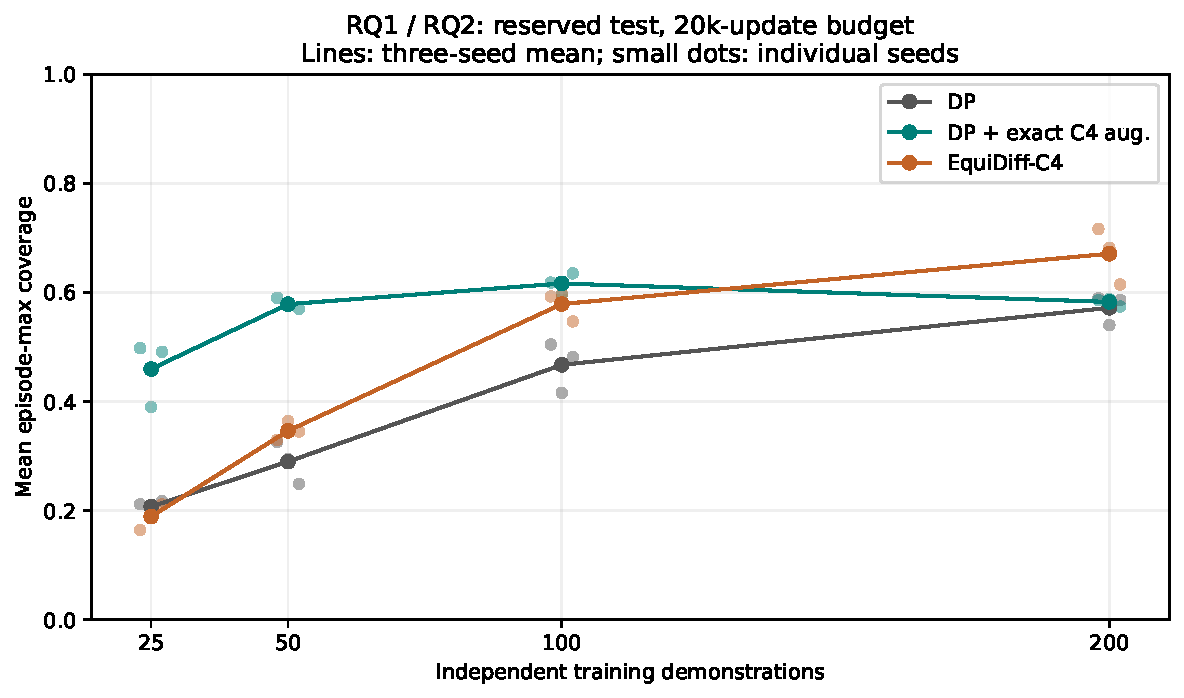
\includegraphics[width=0.88\linewidth]{rq1_rq2_test.pdf}
\caption{Data-efficiency curves on the reserved test set. Lines show three-seed
means; smaller points show individual training seeds. All arms use the
20k-update primary protocol.}
\label{eqstudy:fig:main}
\end{figure}

\begin{table}[t]
\centering
\caption{Paired primary-coverage differences with unadjusted 95\% bootstrap
intervals. Positive values favor EquiDiff-$C_4$.}
\label{eqstudy:tab:deltas}
\resizebox{\linewidth}{!}{%
\begin{tabular}{rcc}
\toprule
Demos & EquiDiff minus DP & EquiDiff minus exact augmentation \\
\midrule
25  & $-0.0183\;[-0.0597,\;0.0262]$ & $-0.2705\;[-0.3597,\;-0.1871]$ \\
50  & $+0.0565\;[-0.0220,\;0.1391]$ & $-0.2322\;[-0.3118,\;-0.1512]$ \\
100 & $+0.1115\;[0.0279,\;0.1896]$ & $-0.0377\;[-0.1145,\;0.0260]$ \\
200 & $+0.0991\;[0.0247,\;0.1596]$ & $+0.0884\;[0.0193,\;0.1452]$ \\
\bottomrule
\end{tabular}}
\end{table}

\subsection{RQ2: exact augmentation is a strong baseline}
Exact augmentation outperforms EquiDiff by 0.2705 and 0.2322 coverage at
25 and 50 demonstrations, respectively, with paired intervals excluding zero.
At 100 demonstrations, augmentation retains a higher mean but the difference
is unresolved. At 200 demonstrations, EquiDiff exceeds augmentation by
0.0884 under the primary budget. The pattern is therefore data-dependent:
architectural equivariance does not consistently dominate an augmentation
baseline whose transformations are valid by construction.

This supports H2's motivation without establishing a uniformly null gap.
It also does not numerically reproduce or refute the augmentation gap in
EquiDiff's Appendix I: the tasks, metrics, and optimization settings differ.
The contribution is a controlled within-task comparison, not a subtraction
of our coverage scores from published manipulation success rates.

\paragraph{Sensitivity to additional training.}
Table~\ref{eqstudy:tab:convergence} and
Figure~\ref{eqstudy:fig:convergence} show independent validation curves.
At 200 demonstrations, augmentation improves from 0.5751 at 20k updates to
0.7422 at 60k; EquiDiff improves from 0.6386 to 0.7501. Their mean gap
shrinks from approximately 0.0634 to 0.0080. This indicates that a
fixed-budget advantage need not imply a higher eventual performance ceiling.
Near-equal validation means do not demonstrate equivalence or complete
convergence. These values belong to the independent validation study,
not the primary test curve in Table~\ref{eqstudy:tab:main}.

\begin{table}[t]
\centering
\caption{Independent validation coverage, 20k $\rightarrow$ 60k updates,
averaged over three seeds. These are individual checkpoints from separate
validation curves, not the primary retained-checkpoint test aggregate.}
\label{eqstudy:tab:convergence}
\begin{tabular}{rccc}
\toprule
Demos & DP & DP + exact aug. & EquiDiff-$C_4$ \\
\midrule
25  & $0.1646\to0.1661$ & $0.4215\to0.4700$ & $0.1716\to0.1945$ \\
50  & $0.2254\to0.2310$ & $0.6278\to0.6377$ & $0.3181\to0.4053$ \\
100 & $0.4372\to0.4551$ & $0.6472\to0.7702$ & $0.5322\to0.6260$ \\
200 & $0.5765\to0.5964$ & $0.5751\to0.7422$ & $0.6386\to0.7501$ \\
\bottomrule
\end{tabular}
\end{table}

\begin{figure}[t]
\centering
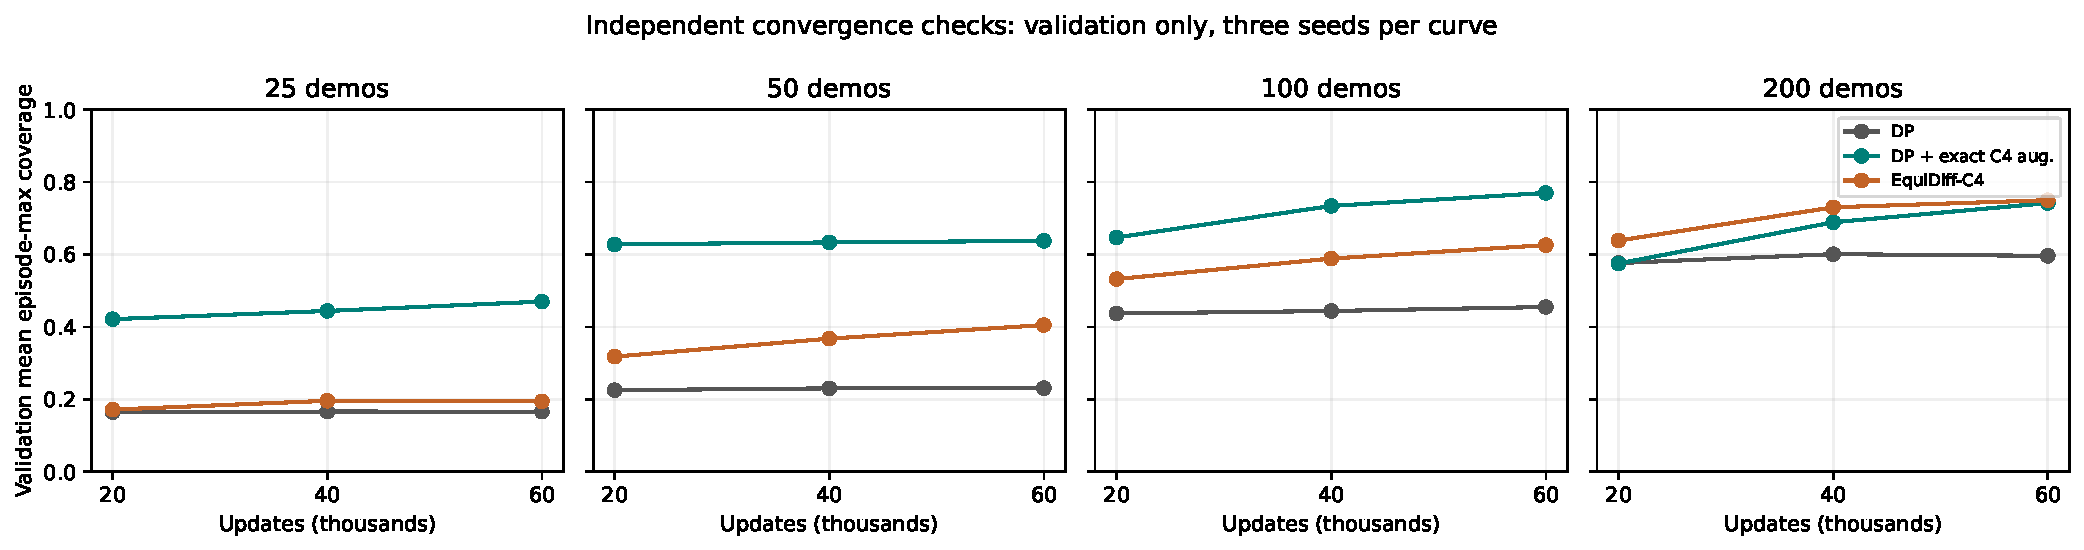
\includegraphics[width=\linewidth]{convergence_validation.pdf}
\caption{Separate validation curves through 60k updates. Each curve averages
three training seeds. Longer training substantially improves the augmented
and equivariant models in several regimes.}
\label{eqstudy:fig:convergence}
\end{figure}

\paragraph{A larger discrete group does not improve this task.}
The $C_8$ variant scores 0.2903 and 0.5826 at 50 and 200 demonstrations,
compared with 0.3465 and 0.6712 for $C_4$. The paired $C_4-C_8$ differences
are 0.0562 [0.0151, 0.1048] and 0.0885 [0.0223, 0.1621]. However,
$45^\circ$ rotations are not exact symmetries of the arena or pixel lattice,
and coordinate-wise DDPM clipping commutes with $C_4$ but not $C_8$.
Parameter counts and runtimes also differ. This is an architecture ablation
on a $C_4$ task, not a controlled demonstration that larger groups are
intrinsically worse or that the sampler is exactly $C_8$-equivariant.

\subsection{RQ3: mismatch is harmful and repairs are partial}
The state-input experiment produces a clear fixed-goal deficit
(Table~\ref{eqstudy:tab:state}). EquiDiff scores 0.4888, compared with
0.7869 for DP: a difference of $-0.2981$ with interval
$[-0.3676,-0.2282]$. Goal input improves coverage by 0.1295
$[0.0631,0.1915]$ over ordinary EquiDiff, and the gate improves it by
0.1335 $[0.0732,0.1938]$. Nevertheless, goal and gate remain below DP
by 0.1686 $[0.0932,0.2448]$ and 0.1646 $[0.1070,0.2248]$,
respectively. The gate-minus-goal interval, $[-0.0543,0.0570]$,
does not resolve a difference between the two repairs.

\begin{table}[t]
\centering
\caption{RQ3 state-input test coverage at 50 demonstrations. Entries are
primary means $\pm$ training-seed standard deviations. Models and budgets
are controlled within the state study, not matched to the image study.}
\label{eqstudy:tab:state}
\resizebox{\linewidth}{!}{%
\begin{tabular}{lcccc}
\toprule
Goal & DP & EquiDiff & EquiDiff + goal & EquiDiff + gate \\
\midrule
Fixed & $\mathbf{0.7869}\pm0.0270$ & $0.4888\pm0.0232$ & $0.6183\pm0.0340$ & $0.6223\pm0.0075$ \\
Rotated & $0.4061\pm0.0123$ & $0.4733\pm0.0340$ & $\mathbf{0.5584}\pm0.0085$ & $0.4771\pm0.0492$ \\
\bottomrule
\end{tabular}}
\end{table}

\begin{figure}[t]
\centering
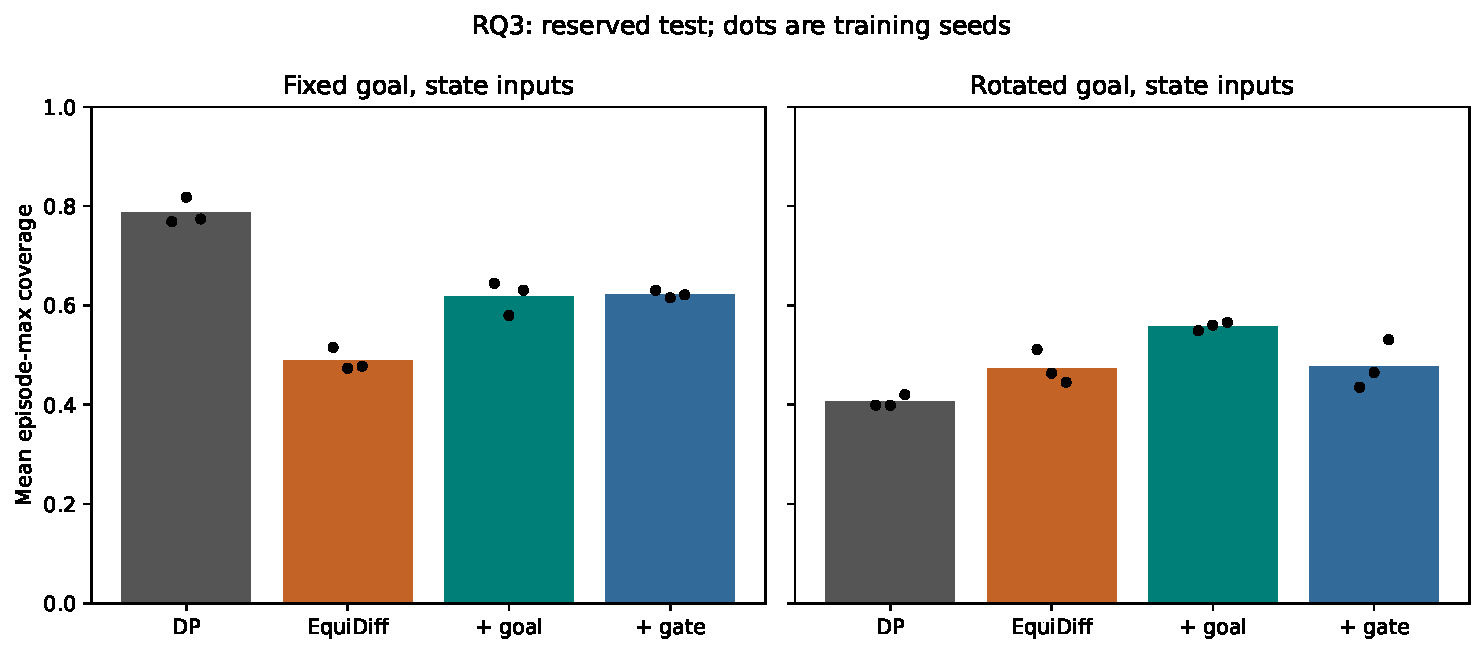
\includegraphics[width=\linewidth]{rq3_state_test.pdf}
\caption{State-input symmetry mismatch and repair. Points denote individual
training seeds. Both modifications improve fixed-goal coverage relative to
ordinary EquiDiff but remain below DP.}
\label{eqstudy:fig:state}
\end{figure}

The failure prediction in H3 is supported, whereas its full-recovery
prediction is not. With rotated goals, goal conditioning achieves the
largest mean, but ordinary EquiDiff's coverage difference from DP has an
interval of $[-0.0149,0.1462]$. Goal input outperforms DP with interval
$[0.0416,0.2582]$, while its coverage difference from ordinary EquiDiff
remains unresolved. Rotating the goal does not make a goal-omitting state
fully informative, and goal conditioning adds information as well as a
compatible transformation reference. These results therefore do not isolate
architecture from observability.

\paragraph{Visible-goal image extension.}
In images, the goal is already visible. The fixed-goal means are 0.3241
for DP, 0.3348 for EquiDiff, and 0.3087 for EquiDiff with the gate; the
corresponding rotated-goal means are 0.2899, 0.3465, and 0.3225.
The fixed-goal EquiDiff-minus-DP coverage interval is
$[-0.0653,0.0876]$, and gate-minus-EquiDiff intervals contain zero in
both conditions. We do not observe the large coverage deficit seen in
the state study, nor a consistent benefit of the gate. This is compatible
with the different information structure: a visible target supplies a
directional reference that is absent from the ordinary state input.
The image extension is exploratory and should not be pooled with the
hidden-goal state experiment as a second confirmation of the same mechanism.

\section{Discussion and Limitations}
\label{eqstudy:sec:discussion}
\paragraph{What the experiments establish.}
The results support a conditional view of equivariance. Exact augmentation
is highly competitive and superior in the smallest data regimes studied.
Architectural advantages at larger data sizes depend on the training budget,
and a mismatched symmetry constraint can impose a substantial cost. Adding
a task reference or allowing symmetry breaking helps, but neither guarantees
recovery. The results do not imply that the original manipulation results
are invalid or that augmentation is universally preferable.

\paragraph{Coverage is not task success.}
Absolute success rates are modest under the primary image budget
(Table~\ref{eqstudy:tab:success}). This is a relative-performance study, not
a demonstration of deployment-ready reliability. Fixed-goal state success
rates are 34.89\%, 5.67\%, 17.00\%, and 18.89\% for DP, EquiDiff,
goal, and gate, consistent with partial recovery. In fixed-goal images,
DP and EquiDiff have success rates of 6.44\% and 1.33\%, despite close
coverage means. Conclusions must remain metric-specific.

\begin{table}[t]
\centering
\caption{Primary image-policy success rates, using episode coverage $>0.95$.
Percentages average the same seeds and retained checkpoints as the primary
coverage metric.}
\label{eqstudy:tab:success}
\begin{tabular}{rccc}
\toprule
Demos & DP & DP + exact aug. & EquiDiff-$C_4$ \\
\midrule
25 & 0.11\% & 2.00\% & 0.33\% \\
50 & 1.00\% & 3.78\% & 2.33\% \\
100 & 1.33\% & 1.11\% & 5.89\% \\
200 & 2.67\% & 0.78\% & 11.89\% \\
\bottomrule
\end{tabular}
\end{table}

\paragraph{Experimental scope.}
The evidence is limited to one planar task family, three training seeds,
and 25 base test states. Equal update counts do not equalize compute or
optimization difficulty. Neither 20k nor 60k establishes full convergence.
The constructed renderer and discrete symmetry do not establish continuous
rotation equivariance for real camera observations. Goal input changes
observability, and state and image results are not directly comparable.
Supplementary experiments use different GPU/PyTorch environments, whose
provenance is retained. The mean over three retained checkpoints is distinct
from a full max-over-training metric. Single-seed official-reference checks
are not substituted for the controlled baselines.

\paragraph{Optional E4 and reproducibility.}
The proposal explicitly labels MimicGen D0-to-D1/D2 evaluation as
\emph{Optional E4}, separate from RQ1--RQ3, and permits dropping it when
compute is insufficient. The current implementation selects the Square
task family. Its final transfer results are unavailable at this snapshot
and are excluded from every claim and table here. Completed main-study
evidence includes 78 test runs and 36 independent validation runs, with
three checkpoints and 100 episodes per checkpoint. The 34,200 stored
checkpoint--episode records are repeated measurements rather than
independent statistical samples. Per-run provenance, source hashes,
episode-level scores, and the CPU analysis script accompany this report.

\section{Conclusion}
We evaluated equivariant diffusion policies in a planar-pushing testbed
designed to separate valid augmentation from architectural symmetry and
to expose task-dependent symmetry mismatch. The proposed low-data advantage
over DP was not established at 25 or 50 demonstrations, while exact
augmentation outperformed the equivariant model in both regimes. Advantages
at larger data sizes depended on optimization budget. A fixed goal omitted
from state input produced a large equivariant-policy deficit; explicit goal
input and a learnable world reference provided partial recovery. These
findings motivate choosing symmetry constraints jointly with task
observability and training resources, rather than treating equivariance
as a universal guarantee of data efficiency.
